\documentclass[10pt]{beamer}

%% Based on the original theme by Matthias Vogelgesang

\usetheme[progressbar=frametitle]{metropolis}
\usepackage{appendixnumberbeamer}

\usepackage{booktabs}
\usepackage[scale=2]{ccicons}

\usepackage{pgfplots}
\usepgfplotslibrary{dateplot}

\usepackage{xspace}
\newcommand{\themename}{\textbf{\textsc{metropolis}}\xspace}

%%%%%%%%%%%%%%%%%%%%%%%%%%%%
%% UNCC Theme Adjustments %%
%%%%%%%%%%%%%%%%%%%%%%%%%%%%
\definecolor{CanvasBG}{HTML}{FAFAFA}

% From the official style guide
\definecolor{UnccGreen}{HTML}{005035}
\definecolor{UnccLightGreen}{HTML}{C3D7A4}
\definecolor{UnccGold}{HTML}{A49665}
\definecolor{UnccOrange}{HTML}{F3901D}
\definecolor{UnccLightYellow}{HTML}{899064}
\definecolor{UnccBlue}{HTML}{007377}
\definecolor{UnccPink}{HTML}{DE3A6E}
\definecolor{White}{HTML}{FFFFFF}
\definecolor{LightGray}{HTML}{F1E6B2}

\setbeamercolor{frametitle}{bg=UnccGreen}
\setbeamercolor{progress bar}{bg=UnccGold, fg=UnccGreen}
\setbeamercolor{alerted text}{fg=UnccOrange}

\setbeamercolor{block title}{bg=UnccGreen, fg=White}
\setbeamercolor{block title example}{bg=UnccBlue, fg=White}
\setbeamercolor{block title alerted}{bg=UnccPink, fg=White}
\setbeamercolor{block body}{bg=LightGray}

\metroset{titleformat=smallcaps, progressbar=foot}

\makeatletter
\setlength{\metropolis@progressinheadfoot@linewidth}{2pt}
\setlength{\metropolis@titleseparator@linewidth}{2pt}
\setlength{\metropolis@progressonsectionpage@linewidth}{2pt}
%%%%%%%%%%%%%%%%%%%%%%%%%%%%
%% UNCC Theme Adjustments %%
%%%%%%%%%%%%%%%%%%%%%%%%%%%%

\title{3D Environment Modeling for Falsification and Beyond with Scenic 3.0}
\author{
    Eric Vin, Shun Kashiwa, Matthew Rhea, Daniel J. Fremont, Edward Kim, Tommaso Dreossi, Shromona Ghosh, Xiangyu Yue, Alberto L. Sangiovanni-Vincentelli, and Sanjit A. Seshia
}
\institute[University of L'Aquila]{
    \textbf{Presented by: Adam Bouafia}\\
    University of L'Aquila\\
    \textbf{Professor: Igor Melatti}\\
    \begin{center}
        
\includegraphics[width=3cm]{uni_logo.png}
    \end{center}
}
\date{}

\begin{document}

\maketitle

\begin{frame}{Table of contents}
  \setbeamertemplate{section in toc}[sections numbered]
  \tableofcontents
\end{frame}
\section{Summary}

\begin{frame}{Summary}
    \begin{itemize}
        \item \textbf{Introduction:} Discusses the challenges of designing CPS, the need for formal models, and how Scenic addresses these challenges. (p. 2)

        \item \textbf{Limitations of Scenic 2.0:} Explains the limitations of Scenic 2.0, such as restriction to 2D environments and the use of bounding boxes. (p. 4)
        \item \textbf{Differences Between Scenic 2.0 and Scenic 3.0:} Highlights the key differences, such as basic syntax changes, support for 3D geometry, improved object representation, comprehensive LTL support, and enhanced error handling with new syntax features. (p. 7)
                \item \textbf{Scenic 3.0 vs. Other Tools:} Compares Scenic to rule/grammar-based tools, probabilistic programming languages, and ML-based scene generation tools, highlighting its unique advantages. (p. 10)

    \end{itemize}
\end{frame}

\begin{frame}{Summary (cont.)}
    \begin{itemize}
            \item \textbf{Key Innovations in Scenic 3.0:} Covers new features like 3D geometry, mesh shapes and regions, precise visibility, temporal requirements, and a rewritten parser. (p. 13)
        \item \textbf{Case Studies:} Presents two case studies on robot vacuum falsification and constrained data generation for an autonomous vehicle. (p. 22)
        \item \textbf{Impact on Formal Methods:} Discusses how Scenic 3.0 extends the scope of formal verification and analysis. (p. 30)
        \item \textbf{Broader Applications:} Describes the broader applications of Scenic 3.0 in training data generation, scenario-based testing, and simulation. (p. 31)
        \item \textbf{Conclusion:} Summarizes the key contributions of Scenic 3.0. (p. 32)
        \item \textbf{Future Directions:} Outlines future directions for Scenic 3.0. (p. 33)
    \end{itemize}
\end{frame}

\section[Intro]{Introduction}

\begin{frame}{Introduction}
    \textbf{The Challenge:} Designing safe and reliable cyber-physical systems (CPS) like autonomous vehicles is difficult due to the complexity and diversity of real-world environments.\\
    \textbf{The Need:} Formal models are essential to accurately represent these environments for rigorous verification and analysis.\\
    \textbf{Scenic to the Rescue:} Scenic, a probabilistic programming language, offers a readable and precise way to model CPS environments.
\end{frame}



\section{Limitations of Scenic 2.0}

\begin{frame}{Limitations of Scenic 2.0}  
    \textbf{Scenic 2.0 Limitations:}\\
    \begin{itemize}
        \item Restricted to 2D environments, limiting its applicability to certain domains (e.g., aerial vehicles, underwater robots).
        \item Used bounding boxes for object representation, leading to inaccurate collision detection and visibility checks.
    \end{itemize}
\end{frame}

\begin{frame}{Limitations of Scenic 2.0 (cont.)}  
    \begin{figure}
        \centering
        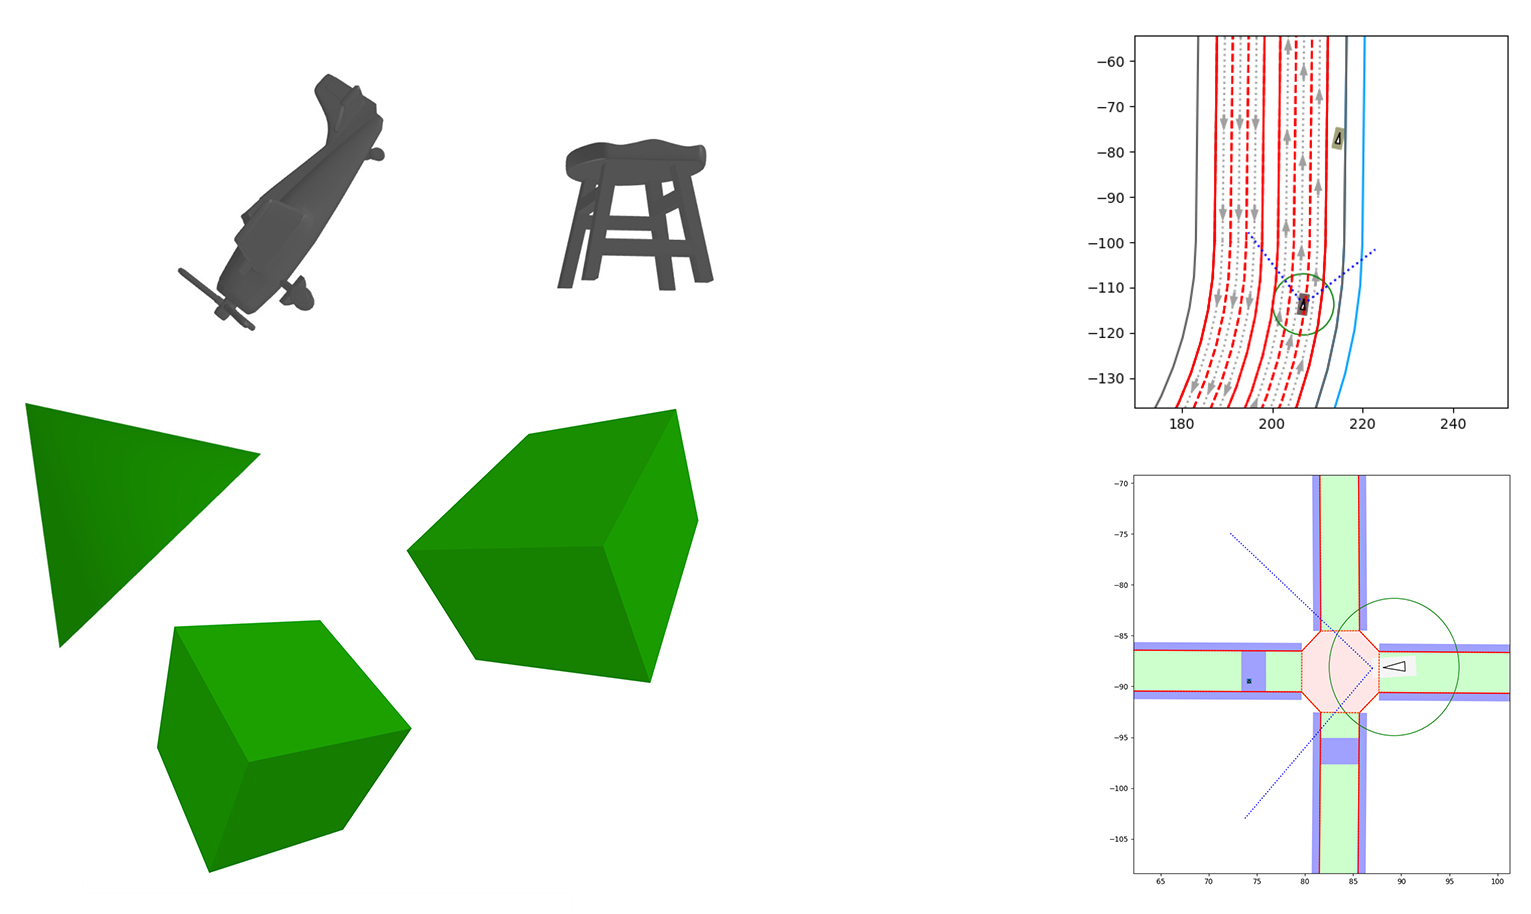
\includegraphics[width=1\linewidth]{2D_vs_3D.png}
        \caption{3D vs 2D environments}
        \label{fig:2d-vs-3d}
    \end{figure}
\end{frame}

\section{Differences Between Scenic 2.0 and Scenic 3.0}

\begin{frame}{1. Basic Syntax: Additional Z-axis parameter and extended facing direction}
\textbf{Scenic 2.0:}
\begin{itemize}
    \item \texttt{ego = Car at (10, 20), facing 90 deg}
\end{itemize}

\textbf{Scenic 3.0:}
\begin{itemize}
    \item \texttt{ego = Car at (10, 20, 5), facing (90 deg, 0 deg)}
\end{itemize}

In this example, Scenic 3.0 includes the Z-axis parameter \texttt{5} and an extended facing direction that includes an additional angle for 3D orientation.
\end{frame}

\begin{frame}{2. 3D Geometry: Support for true 3D environments}
\textbf{Scenic 2.0:}
\begin{itemize}
    \item \texttt{ego = Car at (10, 20), facing 90 deg}
    \item \texttt{obstacle = Building at (30, 40), facing 0 deg}
\end{itemize}

\textbf{Scenic 3.0:}
\begin{itemize}
    \item \texttt{ego = Car at (10, 20, 5), facing (90 deg, 0 deg)}
    \item \texttt{obstacle = Building at (30, 40, 15), facing (0 deg, 0 deg)}
\end{itemize}

In this example, Scenic 3.0 allows for specifying the Z-axis positions for both the \texttt{Car} and the \texttt{Building}, making it a true 3D environment.
\end{frame}

\begin{frame}{3. Object Representation: Detailed 3D meshes vs bounding boxes}
\textbf{Scenic 2.0:}
\begin{itemize}
    \item \texttt{ego = Car at (10, 20), facing 90 deg}
\end{itemize}

Objects were represented using simple bounding boxes.

\textbf{Scenic 3.0:}
\begin{itemize}
    \item \texttt{ego = Car at (10, 20, 5), facing (90 deg, 0 deg), with mesh "detailed car mesh.obj"}
\end{itemize}

In this example, Scenic 3.0 allows the use of detailed 3D meshes for more accurate object representation.
\end{frame}

\begin{frame}{4. Temporal Logic: Comprehensive LTL support}
\textbf{Scenic 2.0:}
\begin{itemize}
    \item \texttt{monitor (always ego.speed <= 30)}
\end{itemize}

Basic temporal logic support.

\textbf{Scenic 3.0:}
\begin{itemize}
    \item \texttt{monitor (G (ego.speed <= 30) -> F (ego.location == (50, 50, 5)))}
\end{itemize}

In this example, Scenic 3.0 uses comprehensive Linear Temporal Logic (LTL) with operators like \texttt{G} (globally) and \texttt{F} (finally) to express complex temporal conditions.
\end{frame}

\begin{frame}{5. Parser Improvements: Enhanced error handling and new syntax features}
\textbf{Scenic 2.0:}
\begin{itemize}
    \item \texttt{ego = Car at (10, 20), facing 90 deg}
\end{itemize}

Simple syntax with limited error handling.

\textbf{Scenic 3.0:}
\begin{itemize}
    \item \texttt{ego = Car at (10, 20, 5), facing (90 deg, 0 deg)}
    \item \texttt{\# Enhanced syntax features}
    \item \texttt{if (timeofday == "night"):}
    \item \texttt{    ego.headlights.on()}
    \item \texttt{else:}
    \item \texttt{    ego.headlights.off()}
\end{itemize}

In this example, Scenic 3.0 includes enhanced syntax features like conditional statements and improved error handling for more robust and flexible scenario definitions.
\end{frame}

\begin{frame}{Scenic 3.0 vs. Other Tools}
    \begin{itemize}
        \item Unlike rule/grammar-based tools, Scenic offers more control and enforces requirements over generated data.
        \item Unlike probabilistic programming languages, Scenic provides specialized syntax for geometric scenarios and dynamic behaviors.
        \item Unlike ML-based scene generation, Scenic offers more specificity and control.
    \end{itemize}
\end{frame}

\begin{frame}{Scenic 3.0 vs. Other Tools (cont.)}
    \textbf{Scenic vs. Rule/Grammar-Based Tools:}\\
    \begin{itemize}
        \item \textbf{Example:} In rule-based tools, generating scenarios for an autonomous vehicle might involve manually defining the rules for every possible interaction at an intersection. For example, a rule might state that "a car must stop if there is a pedestrian crossing".
        \item \textbf {Scenic's Advantage:} Scenic allows for more flexible scenario generation by using probabilistic programming. We can define probabilistic behaviors and constraints rather than exhaustive rules. For instance, specifying that "the probability of a pedestrian crossing the street within 5 seconds is 0.3," which adds variability and realism to the scenarios.
    \end{itemize}
\end{frame}

\begin{frame}{Scenic 3.0 vs. Other Tools (cont.)}
    \textbf{Scenic vs. Probabilistic Programming Languages:}\\
    \begin{itemize}
        \item \textbf{Example:} Probabilistic programming languages like Stan or Pyro are powerful for statistical modeling but lack specialized syntax for describing geometric and dynamic scenarios crucial for CPS.
        \item \textbf {Scenic's Advantage:} Scenic provides a specialized syntax to define spatial configurations and temporal behaviors directly. For example, you can easily specify that "an object is placed on a surface with a random orientation within specified bounds," which is particularly useful for testing perception algorithms in autonomous vehicles.
    \end{itemize}
\end{frame}

\begin{frame}{Scenic 3.0 vs. Other Tools (cont.)}
    \textbf{Scenic vs. Machine Learning-Based Scene Generation:}\\
    \begin{itemize}
        \item \textbf{Example:} ML-based tools, such as those using Generative Adversarial Networks (GANs), can generate realistic-looking scenes but lack control over specific elements within the scene.
        \item \textbf {Scenic's Advantage:} Scenic offers precise control over each element of the scene. For instance, in a generated urban environment, you can specifically place a stop sign at a particular distance from an intersection and ensure it is visible to the vehicle's sensors under certain conditions, which is critical for testing specific perception capabilities.
    \end{itemize}
\end{frame}

\section{Key Innovations in Scenic 3.0}

\begin{frame}{The Need for 3D in Scenic 3.0}
    \textbf{Why 3D Matters:}\\
    \begin{itemize}
        \item \textbf{Real-World Complexity:} Many CPS operate in 3D spaces.
        \item \textbf{Perception Challenges:} Accurate perception requires understanding occlusion and complex object shapes.
        \item \textbf{Verification Needs:} Formal verification demands precise modeling of 3D geometry and physics.
    \end{itemize}
\end{frame}

\begin{frame}{Scenic 3.0: Key Innovations - 3D Geometry (cont.)}
\begin{figure}
\centering
\includegraphics[width=0.5\linewidth]{syntax.png}
\caption{Object and Point Placement in Scenic 3.0}
\label{fig:syntax}
\end{figure}
\end{frame}

\begin{frame}{Scenic 3.0: Key Innovations - 3D Geometry (cont.)}
  \begin{itemize}
    \item \textbf{Code Example of Line-of-sight-based orientations:}
  \end{itemize}
\begin{figure}
\centering
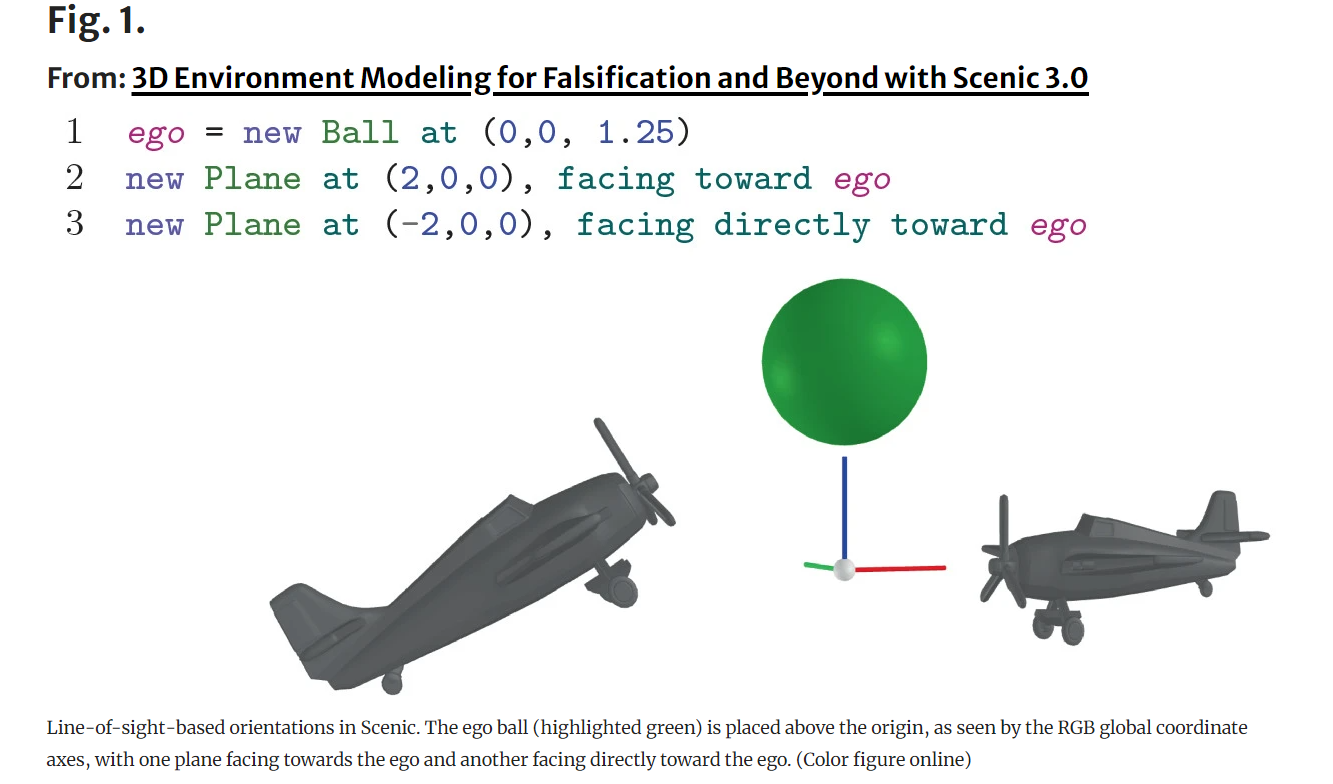
\includegraphics[width=0.7\linewidth]{FIG1.png}
\caption{Line-of-sight-based orientations in Scenic. The ego ball is placed above the origin with one plane facing towards the ego and another facing directly toward the ego.}
\label{fig:line-of-sight}
\end{figure}
\end{frame}

\begin{frame}{Scenic 3.0: Key Innovations - 3D Geometry (cont.)}
    \textbf{Explanation of Line-of-sight-based orientations Example Code:}\\
    \begin{itemize}
        \item \textbf{ego = new Ball at (0,0, 1.25):} This line creates a new object named ego, which is a ball placed at coordinates (0,0,1.25) in the 3D space.
        \item \textbf{new Plane at (2,0,0), facing toward ego:} This line creates a new plane at coordinates (2,0,0). The plane is oriented such that it faces towards the ego ball.
        \item \textbf{new Plane at (-2,0,0), facing directly toward ego:}This line creates another plane at coordinates (-2,0,0). This plane is oriented to face directly toward the ego ball, meaning it adjusts its pitch and yaw to align its front towards the ball.
    \end{itemize}
\end{frame}

\begin{frame}{Scenic 3.0: Key Innovations - 3D Geometry (cont.)}
  \begin{itemize}
    \item \textbf{Code Example of placing a chair on a floor:}
  \end{itemize}
\begin{figure}
\centering
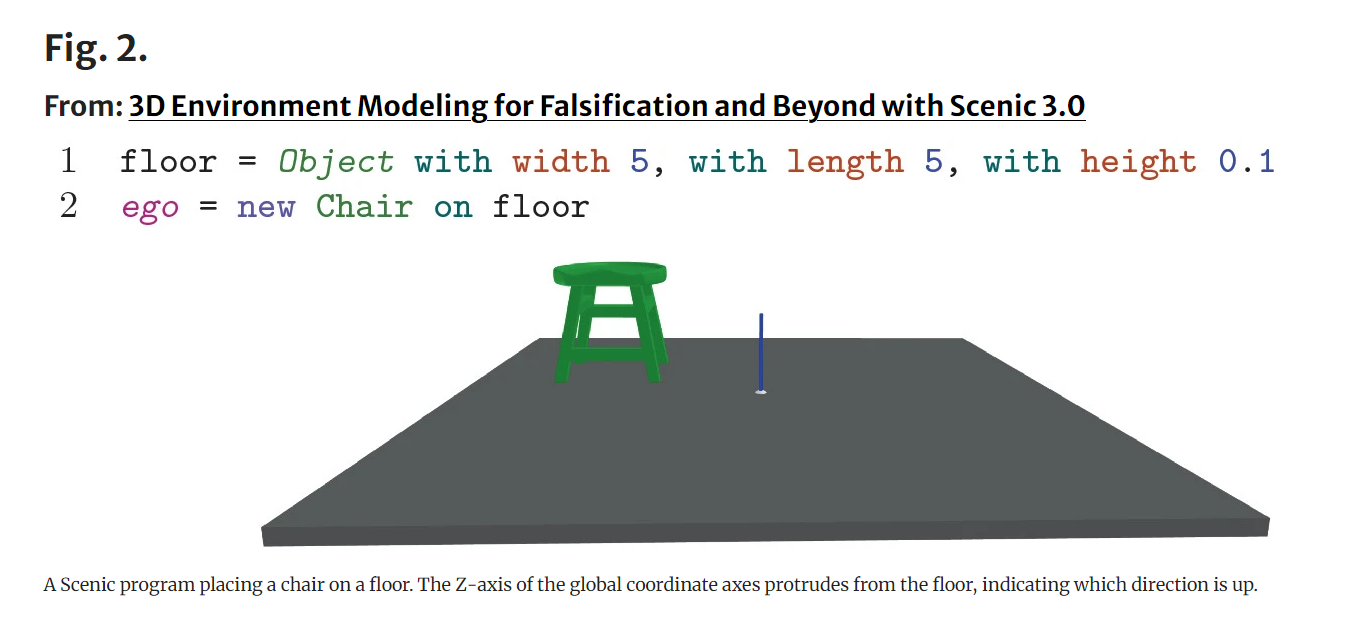
\includegraphics[width=0.7\linewidth]{FIG2.png}
\caption{A Scenic program placing a chair on a floor. The Z-axis of the global coordinate axes protrudes from the floor, indicating which direction is up.}
\label{fig:chair-on-floor}
\end{figure}
\end{frame}

\begin{frame}{Scenic 3.0: Key Innovations - 3D Geometry (cont.)}
    \textbf{Explanation of placing a chair on a floor Example Code:}\\
    \begin{itemize}
        \item \textbf{floor = Object with width 5, with length 5, with height 0.1:} This line creates a new object representing the floor, with specified dimensions (width, length, height).
        \item \textbf{ego = new Chair on floor: }This line creates a new chair object named ego, placing it on top of the floor object.
    \end{itemize}
\end{frame}

\begin{frame}{More on 3D Geometry}
    \textbf{Handling Complex Placements:} Specifiers for placing objects on surfaces, with options for adjusting orientation and position.
    \begin{figure}
        \centering
        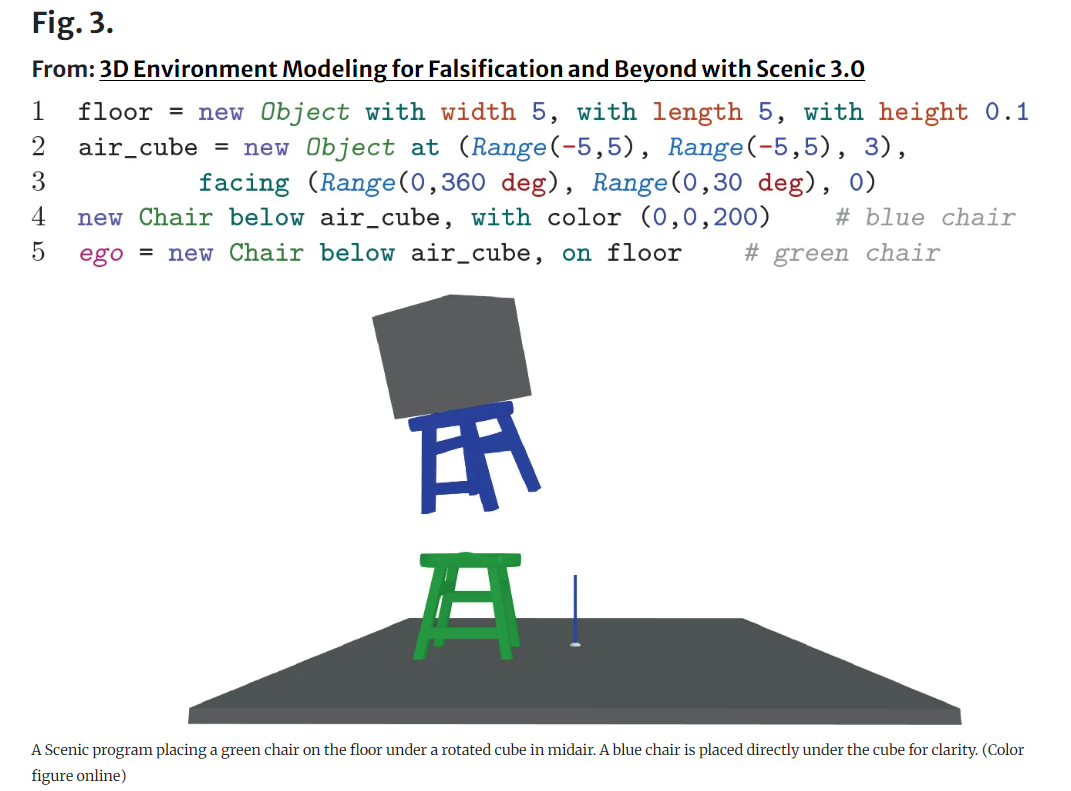
\includegraphics[width=0.6\textwidth]{FIG3.png}
        \caption{A Scenic program placing a green chair on the floor under a rotated cube in midair. A blue chair is placed directly under the cube for clarity.}
        \label{fig:complex-placements}
    \end{figure}
\end{frame}

\begin{frame}{More on 3D Geometry (cont.)}
    \textbf{Explanation of Handling Complex Placement Example Code:}\\
    \begin{itemize}
        \item \textbf{floor = new Object with width 5, with length 5, with height 0.1:} Creates a floor object with specified dimensions.
        \item \textbf{air\_cube = new Object at (Range(-5,5), Range(-5,5), 3), facing (Range(0,360 deg), Range(0,30 deg), 0):} Creates a cube object placed randomly within a range of coordinates in the XY plane at a fixed height of 3 units. The cube faces a random direction within the specified ranges of yaw and pitch angles.
        \item \textbf{new Chair below air\_cube, with color (0,0,200):} Creates a blue chair placed directly below the air\_cube.
        \item \textbf{ego = new Chair below air\_cube, on floor:} Creates a green chair placed directly below the air\_cube and on the floor.
    \end{itemize}
\end{frame}

\begin{frame}{Key Innovations - Mesh Shapes and Regions}
    \textbf{Precise 3D Shapes:} Objects are represented using detailed 3D meshes, not just bounding boxes.
\begin{figure}
\centering
\includegraphics[width=0.7\textwidth]{3d.jpg}
\caption{Example of Precise 3D Shapes.}
\label{fig:3d}
\end{figure}
\end{frame}

\begin{frame}{Key Innovations - Mesh Shapes and Regions (cont.)}
    \textbf{Example: City Intersection with Aerial Surveillance}

    \begin{figure}
        \centering
        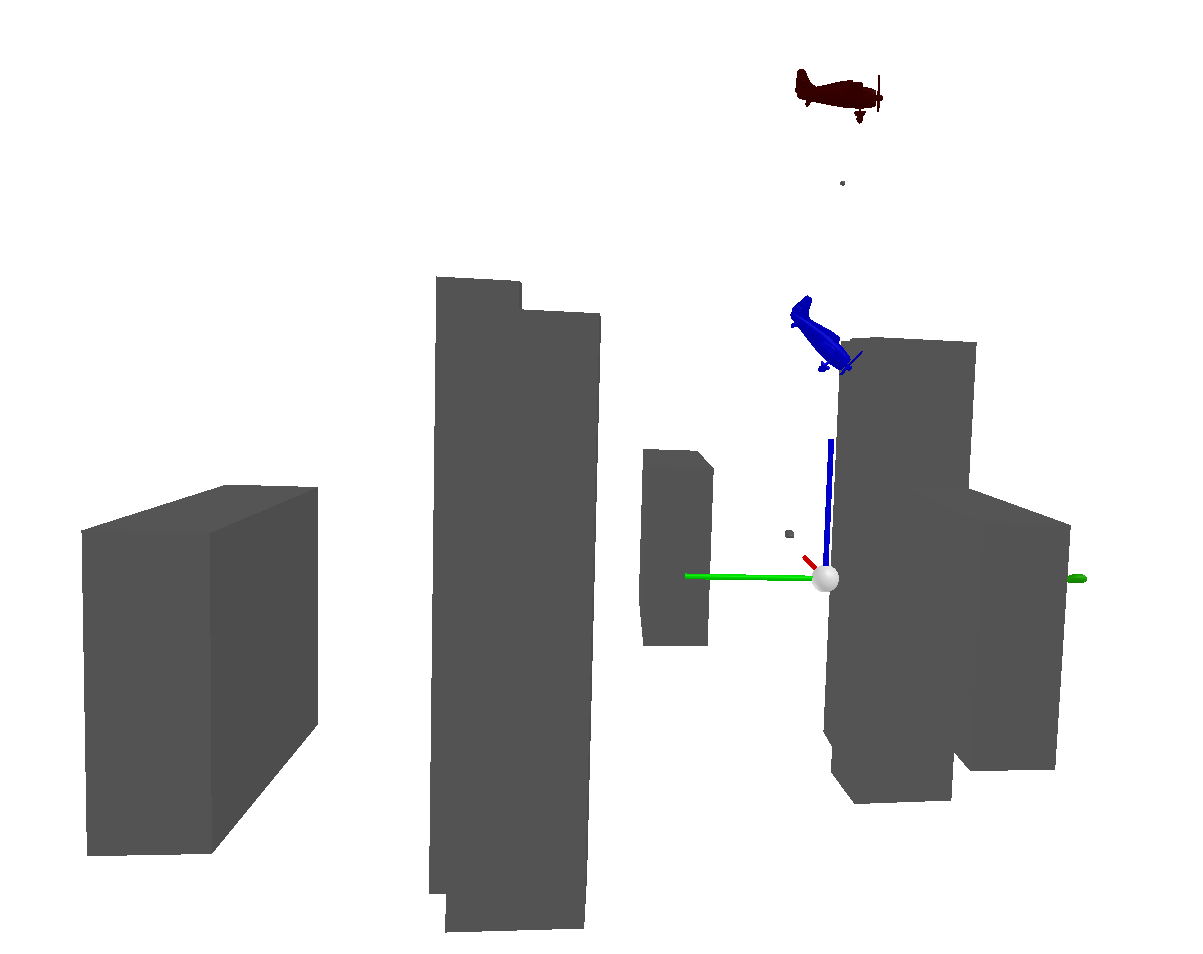
\includegraphics[width=0.65\linewidth]{City_Intersection_with_Aerial_Surveillance.png} 
        \caption{A complex 3D scene created in Scenic 3.0, demonstrating mesh-based shapes, regions, and precise visibility for aerial surveillance in a city intersection.}
        \label{fig:city-intersection}
    \end{figure}
\end{frame}

\begin{frame}{Key Innovations - Precise Visibility}
    \textbf{Accurate Collision Detection:} Mesh-based collision checks ensure realistic object interactions.\\
    \textbf{Mesh Regions:} Define surfaces and volumes for precise object placement and sampling as it uses the Trimesh library to handle the 3D meshes which enable accurate collisions and containment checks.\\
    \textbf{Ray Tracing:} Visibility checks use ray tracing to account for occlusion and complex shapes.
\end{frame}

\begin{frame}{Key Innovations - Temporal Requirements}
\textbf{Realistic Sensor Modeling:} Supports various view cones (e.g., cameras, LiDAR) for accurate sensor simulation.\\
\textbf{Performance Optimizations:} Heuristics for efficient ray tracing in simple cases.\\
\textbf{Temporal Requirements:} Express complex temporal constraints using Linear Temporal Logic (LTL).
\end{frame}

\begin{frame}{Key Innovations - Rewritten Parser and Visualization}
\textbf{Rewritten Parser:} Improved parser based on a formal grammar for better error handling and extensibility as it is based on a Parsing Expression Grammar (PEG) which improves error handling and allows for easier extension of the language.
\begin{itemize}
\item \textbf{Code example:}
    \begin{figure}
    \centering
      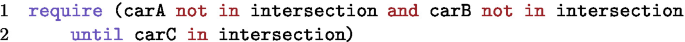
\includegraphics[width=1\linewidth]{FIG8.png}
        \caption{Scenic 3 extends to arbitrary properties in Linear Temporal Logic, allowing natural properties like this to be concisely expressed:}
        \label{fig:Linear-Temporal-Logic}
    \end{figure}
\end{itemize}
\end{frame}

\section{Case Studies}

\begin{frame}{Case Study 1: Robot Vacuum Falsification}
    \textbf{Goal:} Evaluate the performance of a robot vacuum in cluttered environments.\\
    \textbf{Scenic 3.0's Role:} Generate diverse 3D room layouts with varying object placements.\\
    \textbf{Specification:} The robot must clean at least a third of the room within 5 minutes.
\end{frame}

\begin{frame}{Case Study 1: Results and Analysis}
\textbf{Results:} Revealed limitations in the vacuum's navigation and cleaning capabilities, particularly in the presence of many obstacles.
    \begin{figure}
        \centering
        \resizebox{0.7\textwidth}{!}{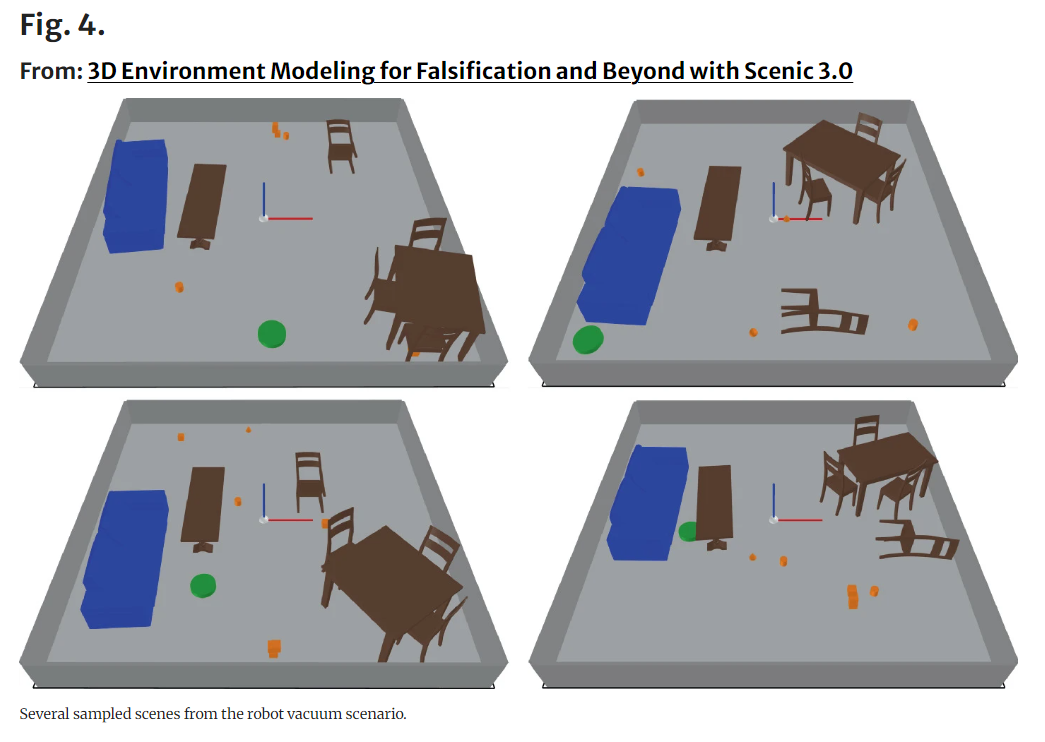
\includegraphics[width=0.7\textwidth]{FIG4.png}} 
        \caption{Several sampled scenes from the robot vacuum scenario.}
        \label{fig:robot-vacuum}
    \end{figure}
\end{frame}

\begin{frame}{Case Study 1: Results and Analysis (cont.)} 
\textbf{Results:} We tested the default controller for the vacuum against 0, 1, 2, 4, 8, and 16-toy variants of our Scenic scenario, running 25 simulations for each variant.\\For each simulation, we computed the robustness value of our spec.\\The average values are plotted in Fig. 5, showing a clear decline as the number of toys increases. Many of the runs actually falsified : up to 44\% with 16 toys.
\end{frame}

\begin{frame}{Case Study 1: Results and Analysis (cont.)}
    \begin{figure}
        \centering
        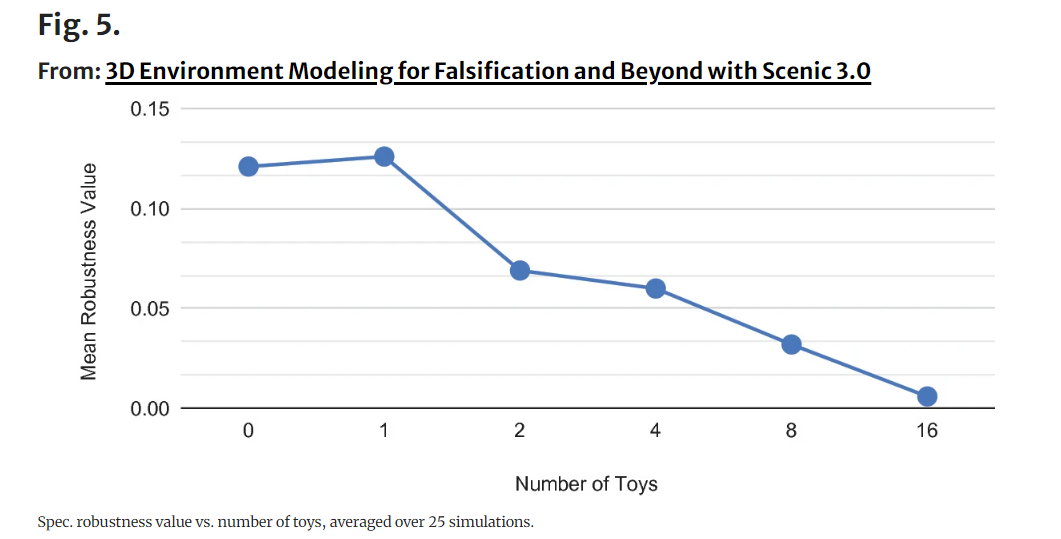
\includegraphics[width=0.7\textwidth]{FIG5.png}
        \caption{Spec. robustness value vs. number of toys, averaged over 25 simulations.}
        \label{fig:case-study-1}
    \end{figure}
\end{frame}

\begin{frame}{Case Study 1: Why Scenic 3.0 Matters}
  \textbf{Why Scenic 3.0 Matters:}
  \begin{itemize}
\item \textbf{3D Modeling:} Accurately represents the vacuum's interactions with furniture and toys.
\item \textbf{Complex Scenarios:} Generates challenging scenarios with objects placed on top of each other or in tight spaces.
\item \textbf{Diverse Layouts:} Samples from a wide range of room configurations for comprehensive testing.
  \end{itemize}
\end{frame}

\begin{frame}{Case Study 2: Constrained Data Generation for an Autonomous Vehicle}
\textbf{Goal:} Test an autonomous vehicle's perception system in an urban intersection with occluding buildings.\\
\textbf{Scenic 3.0's Role:} Create realistic 3D models of the intersection, including buildings, parked cars, and pedestrians.
\end{frame}

\begin{frame}{Case Study 2: Results and Analysis}
  \textbf{Specification:} The crossing car should not be visible until it is close to the autonomous vehicle.\\
\textbf{Results:} Produced a dataset of realistic and challenging scenarios for perception system evaluation, highlighting the importance of accurate occlusion modeling.

\begin{figure}
\centering
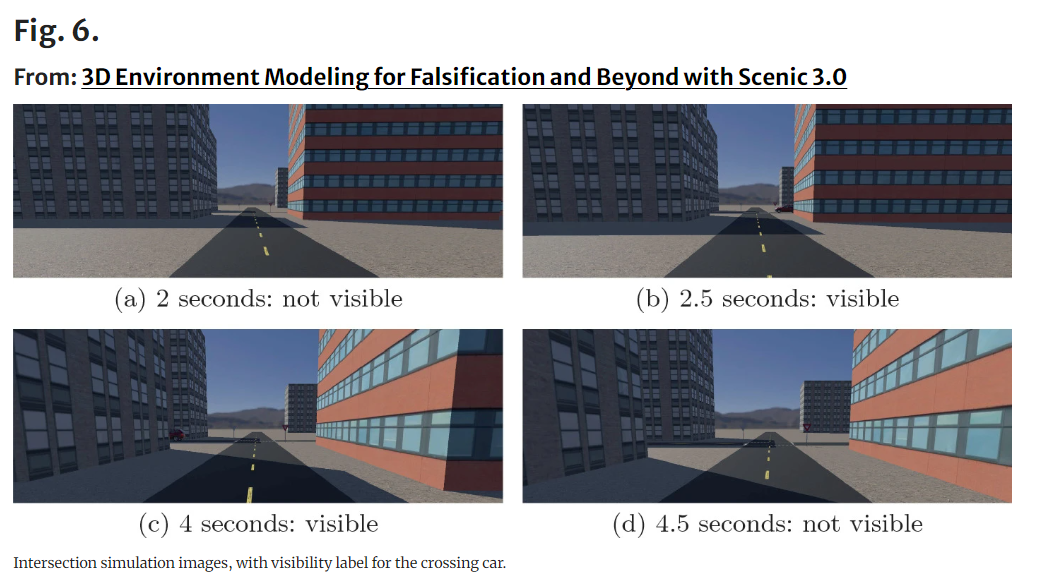
\includegraphics[width=0.7\textwidth]{FIG6.png}
\caption{Intersection simulation images, with visibility label for the crossing car.}
\label{fig:intersection}
\end{figure}
\end{frame}

\begin{frame}{Case Study 2: Why Scenic 3.0 Matters}
\textbf{Why Scenic 3.0 Matters:}
\begin{itemize}
\item \textbf{Precise Visibility:} Accurately models occlusion caused by buildings and other objects.
\item \textbf{Temporal Requirements:} Ensures scenarios meet specific criteria (e.g., car not visible until a certain distance).
\item \textbf{Diverse Scenarios:} Generates a wide range of challenging situations for robust perception system testing.
\end{itemize}
\end{frame}

\section{Impact and Applications}

\begin{frame}{Scenic 3.0's Impact on Formal Methods}
    \textbf{Extends Scope:} Enables formal verification and analysis in new domains (e.g., aerial vehicles, underwater robots).\\
    \textbf{Realistic Scenarios:} Generates more realistic and challenging scenarios for testing and validation.\\
    \textbf{Improved Accuracy:} Precise 3D modeling and visibility checks lead to more accurate results.
\end{frame}

\begin{frame}{Broader Applications of Scenic 3.0}
    \textbf{Training Data Generation:} Create large, diverse datasets for machine learning models.\\
    \textbf{Scenario-Based Testing:} Design and execute comprehensive test suites for CPS.\\
    \textbf{Simulation and Visualization:} Visualize and explore complex 3D environments.
\end{frame}

\section{Limitations}
\begin{frame}{Limitations of Scenic 3.0 (1/3)}
  \begin{itemize}
    \item \textbf{Learning Curve:} 
    \begin{itemize}
      \item Mastering the syntax and semantics of Scenic, especially for complex 3D scenarios, may require significant effort for new users.
    \end{itemize}
    \item \textbf{Simulator Compatibility:} 
    \begin{itemize}
      \item \textbf{Carla Simulator:} 
      \begin{itemize}
        \item To use Carla alongside Scenic, it requires at least 8 GB of VRAM and 32 GB of RAM.
        \item Ensure we have Carla version 0.9.11 or later for full compatibility.
          \end{itemize}
      \item \textbf{GTA V Simulator:} 
      \begin{itemize}
        \item Integration with GTA V requires a specific older version (from approximately 4 years ago).
        \item The plugin DeepGTAV, which facilitates this integration, has not been updated for several years.
        \item Rockstar does not permit such experimentation with newer versions of the game.
      \end{itemize}
    \end{itemize}
  \end{itemize}
\end{frame}

\begin{frame}{Limitations of Scenic 3.0 (2/3)}
    \item \textbf{Limited Documentation and Community Support:} 
    \begin{itemize}
      \item There might be limited documentation and community support compared to more mainstream tools.
    \end{itemize}
        \item \textbf{Performance Issues:} 
    \begin{itemize}
      \item Real-time simulation can suffer from performance issues, especially when simulating highly dynamic environments with many interactive agents.
    \end{itemize}
\end{frame}

\begin{frame}{Limitations of Scenic 3.0 (3/3)}
  \begin{itemize}
    \item \textbf{Integration Challenges:} 
    \begin{itemize}
      \item Integrating Scenic with other custom or less popular simulators can be challenging and might require significant custom development efforts.
    \end{itemize}
    \item \textbf{Debugging Complexity:} 
    \begin{itemize}
      \item Debugging scenarios in Scenic can be complex due to the probabilistic nature of the scenarios, making it harder to reproduce and diagnose issues.
    \end{itemize}
    \item \textbf{Licensing and Usage Restrictions:} 
    \begin{itemize}
      \item Some simulators that Scenic integrates with may have licensing and usage restrictions, which can limit the scenarios that can be legally tested or shared.
    \end{itemize}
  \end{itemize}
\end{frame}

\section{Conclusion}

\begin{frame}{Conclusion}
    \textbf{Key Takeaway:} Scenic 3.0 is a powerful tool for modeling, analyzing, and verifying CPS in complex 3D environments.\\
    \textbf{Contributions:}
    \begin{itemize}
        \item Native 3D syntax and specifiers
        \item Precise mesh-based shapes and regions
        \item Ray tracing-based visibility
        \item Temporal requirements with LTL
        \item Rewritten parser
    \end{itemize}
\end{frame}

\begin{frame}{Future Directions}
    \textbf{3D Scenario Optimization:} Develop algorithms to automatically optimize 3D scenarios for specific verification goals.\\
    \textbf{Drone Applications:} Explore the use of Scenic 3.0 for modeling and verifying drone behaviors in complex environments.\\
    \textbf{Custom Specifiers and Pruning:} Allow users to define their own specifiers and pruning techniques for greater flexibility.
\end{frame}

\begin{frame}{Future Work and Tutorial}
    \begin{itemize}
        \item \textbf{Hands-on Tutorial at CVPR 2024:}\\ On June 17 from 9am-12pm PDT, It will be a hands-on tutorial on Scenic 3.0 at CVPR 2024 in Seattle. \\
        A video will be available afterward. More information at: \url{https://scenic-lang.org/cvpr24} 
    \end{itemize}
\end{frame}
\end{document}
